\documentclass[aspectratio=169]{beamer}

% -------------------------
% Packages
% -------------------------
\usepackage[utf8]{inputenc}
\usepackage{graphicx}
\usepackage{amsmath, amssymb}
\usepackage{booktabs}
\usepackage{tcolorbox}
\usepackage{tikz}
\definecolor{questionbg}{RGB}{235, 244, 255}
\definecolor{questionframe}{RGB}{44, 95, 173}
\definecolor{plainbg}{RGB}{241, 249, 241}
\definecolor{plainframe}{RGB}{44, 122, 70}
\definecolor{notationbg}{RGB}{255, 248, 230}
\definecolor{notationframe}{RGB}{176, 118, 0}

\newtcolorbox{questionbox}{
  colback=questionbg,
  colframe=questionframe,
  boxrule=0.7pt,
  arc=1mm,
  fontupper=\small,
  left=1mm,
  right=1mm,
  top=0.4mm,
  bottom=0.4mm
}

\newtcolorbox{plainbox}{
  colback=plainbg,
  colframe=plainframe,
  boxrule=0.7pt,
  arc=1mm,
  fontupper=\small,
  left=1mm,
  right=1mm,
  top=0.4mm,
  bottom=0.4mm
}

\newtcolorbox{notationbox}{
  colback=notationbg,
  colframe=notationframe,
  boxrule=0.7pt,
  arc=1mm,
  fontupper=\small,
  left=1mm,
  right=1mm,
  top=0.4mm,
  bottom=0.4mm
}

\newcommand{\keyquestion}[1]{%
  \begin{questionbox}
  \textbf{Question:} #1
  \end{questionbox}
}

\newcommand{\plainidea}[1]{%
  \begin{plainbox}
  \textbf{Main idea:} #1
  \end{plainbox}
}

\newcommand{\notationblock}[1]{%
  \begin{notationbox}
  \textbf{Symbols used on this slide}\\
  #1
  \end{notationbox}
}

\newcommand{\exercisebreakcontent}[1]{%
  \begin{center}
  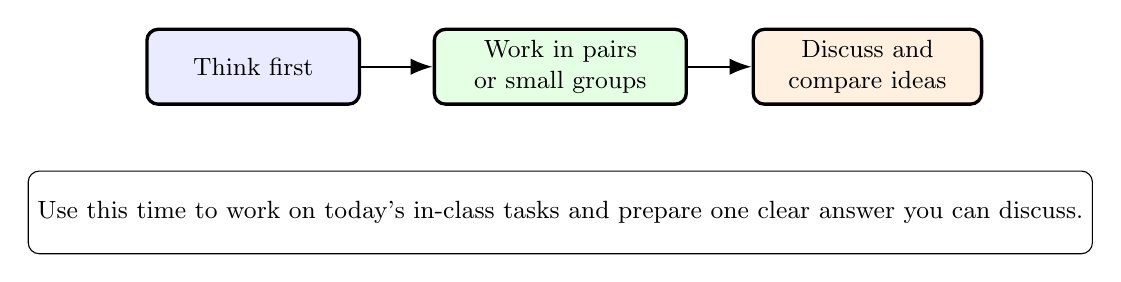
\begin{tikzpicture}[>=Latex, every node/.style={font=\small}]
    \node[draw, rounded corners, very thick, fill=blue!8, minimum width=2.7cm, minimum height=0.95cm, align=center] (think) at (-3.9,0.9) {Think first};
    \node[draw, rounded corners, very thick, fill=green!10, minimum width=3.2cm, minimum height=0.95cm, align=center] (work) at (0,0.9) {Work in pairs\\or small groups};
    \node[draw, rounded corners, very thick, fill=orange!12, minimum width=2.9cm, minimum height=0.95cm, align=center] (share) at (3.9,0.9) {Discuss and\\compare ideas};
    \draw[-{Latex[length=2.8mm]}, thick] (think) -- (work);
    \draw[-{Latex[length=2.8mm]}, thick] (work) -- (share);
    \node[draw, rounded corners, fill=white, minimum width=9.4cm, minimum height=1.05cm, align=center] at (0,-0.95) {Use this time to work on today's in-class tasks and prepare one clear answer you can discuss.};
  \end{tikzpicture}
  \end{center}
  \plainidea{#1}
}

\usepackage{hyperref}
\usetikzlibrary{positioning,arrows.meta,fit}

% -------------------------
% Theme
% -------------------------
\usetheme{Madrid}
\usecolortheme{default}
\setbeamertemplate{navigation symbols}{}

% -------------------------
% Per-slide reference footer
% -------------------------
\newcommand{\defaultdeckrefs}{AIMA4e Ch.10 pp.314--343; Poole3e Ch.16--17 pp.701--766; doi:10.1016/j.cosrev.2026.100902}
\newcommand{\currentsliderefs}{\defaultdeckrefs}
\newcommand{\setslideref}[1]{\gdef\currentsliderefs{#1}}
\addtobeamertemplate{footline}{}{%
  \begin{beamercolorbox}[wd=\paperwidth,leftskip=0.4em,rightskip=0.4em,ht=2.8ex,dp=0.9ex]{author in head/foot}
    \tiny\textbf{Refs: }\currentsliderefs
  \end{beamercolorbox}
}

% -------------------------
% Metadata
% -------------------------
\title[EBU6505 B3 D4]{EBU6505 -- Reasoning and Agents\\Block 3, Day 4 -- Knowledge Graphs in Modern AI}
\author{Dr Riasat Islam}
\institute{Queen Mary University of London}
\date{}

% -------------------------
% TikZ styles
% -------------------------
\tikzset{
  flowarrow/.style={-{Latex[length=2.8mm]}, thick},
  entity/.style={draw, rounded corners, very thick, fill=blue!8, minimum width=2.3cm, minimum height=0.95cm, align=center},
  entity2/.style={draw, rounded corners, very thick, fill=green!10, minimum width=2.3cm, minimum height=0.95cm, align=center},
  stepbox/.style={draw, rounded corners, very thick, fill=blue!6, minimum width=2.5cm, minimum height=0.95cm, align=center},
  stepbox2/.style={draw, rounded corners, very thick, fill=green!8, minimum width=2.5cm, minimum height=0.95cm, align=center},
  note/.style={draw, rounded corners, fill=orange!12, minimum width=2.5cm, minimum height=0.95cm, align=center},
  softbox/.style={draw, rounded corners, fill=white, minimum width=2.7cm, minimum height=0.95cm, align=center},
  relabel/.style={font=\small, fill=white, inner sep=1.5pt}
}

\begin{document}

\setslideref{AIMA4e Ch.10 pp.314--343; Poole3e Ch.16--17 pp.701--766; doi:10.1016/j.cosrev.2026.100902}
\begin{frame}
  \titlepage
\end{frame}

\begin{frame}{What have we covered so far this week?}
\begin{itemize}
  \item MDPs describe sequential decision problems.
  \item Sequential decision models use reward to compare future choices.
  \item Knowledge representation stores facts in a machine-usable form.
  \item Knowledge graphs connect those facts into useful paths.
\end{itemize}
\plainidea{Day 3 showed how to build a graph. Today shows how modern AI systems use that graph.}
\end{frame}

\begin{frame}{What are we going to cover today?}
\begin{itemize}
  \item How knowledge graphs help retrieval, memory, and explanation
  \item How graphs fit inside modern AI systems and agent pipelines
  \item What neuro-symbolic AI means in simple terms
  \item Why MCP, multi-agent systems, and A2A matter in practice
\end{itemize}
\plainidea{The main question today is not how to build a graph. It is how to use a graph well inside a real AI system.}
\end{frame}

\begin{frame}{Resources}
\small
\begin{itemize}
  \item \textit{Artificial Intelligence: Foundations of Computational Agents}, Poole and Mackworth (3rd ed.)
  \item Chapters 16 and 17 -- graph structure and reasoning with linked facts
  \item \textit{Artificial Intelligence: A Modern Approach}, Russell and Norvig (4th ed.)
  \item Chapter 10 -- knowledge representation
  \item Selected review papers on neuro-symbolic AI and agentic AI systems
  \item Full review-paper citations are listed on the next slide
\end{itemize}
\plainidea{Use the textbooks for the foundations. Use the review papers to see how these ideas are used in current systems.}
\end{frame}

\begin{frame}{Review Papers for This Lecture}
\footnotesize
\begin{itemize}
  \item DeLong et al. (2025). \textit{Neurosymbolic AI for Reasoning Over Knowledge Graphs: A Survey}.\\
  \href{https://doi.org/10.1109/TNNLS.2024.3420218}{doi:10.1109/TNNLS.2024.3420218}
  \item Colelough and Regli (2025). \textit{Neuro-Symbolic AI in 2024: A Systematic Review}.\\
  \href{https://doi.org/10.48550/arXiv.2501.05435}{doi:10.48550/arXiv.2501.05435}
  \item Nawaz et al. (2025). \textit{A Review of Neuro-Symbolic AI Integrating Reasoning and Learning for Advanced Cognitive Systems}.\\
  \href{https://doi.org/10.1016/j.iswa.2025.200541}{doi:10.1016/j.iswa.2025.200541}
  \item Hakim et al. (2026). \textit{Neuro-Symbolic Agentic AI: Architectures, Integration Patterns, Applications, and Open Challenges}.\\
  \href{https://doi.org/10.1016/j.cosrev.2026.100902}{doi:10.1016/j.cosrev.2026.100902}
\end{itemize}
\plainidea{These review papers give the broader research picture behind the design ideas discussed in this lecture.}
\end{frame}

\begin{frame}{Learning Outcomes for Today}
By the end of this session, you should be able to:
\begin{itemize}
  \item explain where a knowledge graph adds value in a modern AI stack
  \item compare several simple ways to combine graphs with neural models
  \item explain why tool protocols and multi-agent coordination matter
  \item describe the role of evidence, guardrails, and traceability in agent systems
\end{itemize}
\end{frame}

\begin{frame}{Warm-up Question}
\keyquestion{If an assistant reads only text chunks, what important thing might it miss?}
\begin{columns}[T,onlytextwidth]
  \begin{column}{0.44\textwidth}
    \begin{itemize}
      \item text chunks may contain the right words
      \item but they may not show the exact relation
      \item the answer can become vague or wrong
    \end{itemize}
  \end{column}
  \begin{column}{0.52\textwidth}
    \begin{center}
    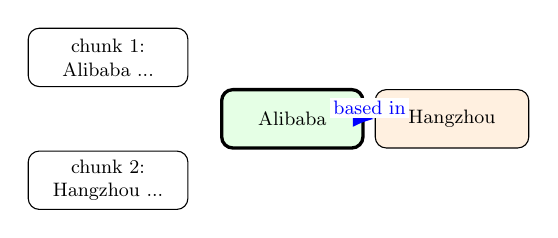
\begin{tikzpicture}[>=Latex, scale=0.78, transform shape, every node/.style={font=\small}]
      \node[softbox, minimum width=2.6cm] (c1) at (0,1.0) {chunk 1:\\ Alibaba ...};
      \node[softbox, minimum width=2.6cm] (c2) at (0,-1.0) {chunk 2:\\ Hangzhou ...};
      \node[entity2] (ali) at (3.0,0) {Alibaba};
      \node[note] (hz) at (5.6,0) {Hangzhou};
      \draw[flowarrow, very thick, blue] (ali) -- node[relabel, above]{based in} (hz);
    \end{tikzpicture}
    \end{center}
  \end{column}
\end{columns}
\plainidea{The graph makes the relation explicit. It shows not just the words, but the exact connection between them.}
\end{frame}

\begin{frame}{Where Does a Knowledge Graph Help?}
\keyquestion{In a modern AI system, where can a knowledge graph add value?}
\begin{center}
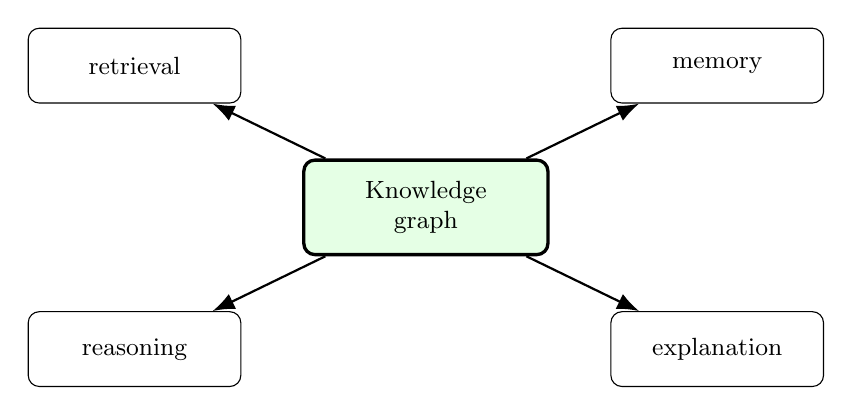
\begin{tikzpicture}[>=Latex, every node/.style={font=\small}]
  \node[entity2, minimum width=3.1cm, minimum height=1.2cm] (kg) at (4.2,0) {Knowledge\\ graph};
  \node[softbox, minimum width=2.7cm] (ret) at (0.5,1.8) {retrieval};
  \node[softbox, minimum width=2.7cm] (mem) at (7.9,1.8) {memory};
  \node[softbox, minimum width=2.7cm] (rea) at (0.5,-1.8) {reasoning};
  \node[softbox, minimum width=2.7cm] (exp) at (7.9,-1.8) {explanation};
  \draw[flowarrow] (kg) -- (ret);
  \draw[flowarrow] (kg) -- (mem);
  \draw[flowarrow] (kg) -- (rea);
  \draw[flowarrow] (kg) -- (exp);
\end{tikzpicture}
\end{center}
\plainidea{The graph helps the system find better evidence, remember facts, reason over paths, and explain answers.}
\end{frame}

\begin{frame}{KGs with RAG}
\keyquestion{How does a knowledge graph improve a retrieval-augmented system?}
\begin{center}
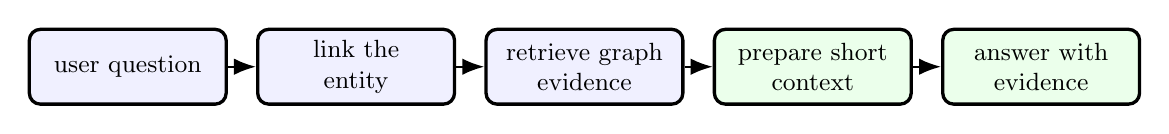
\begin{tikzpicture}[>=Latex, every node/.style={font=\small}]
  \node[stepbox] (q) at (0,0) {user question};
  \node[stepbox] (link) at (2.9,0) {link the\\ entity};
  \node[stepbox] (graph) at (5.8,0) {retrieve graph\\ evidence};
  \node[stepbox2] (ctx) at (8.7,0) {prepare short\\ context};
  \node[stepbox2] (ans) at (11.6,0) {answer with\\ evidence};
  \draw[flowarrow] (q) -- (link);
  \draw[flowarrow] (link) -- (graph);
  \draw[flowarrow] (graph) -- (ctx);
  \draw[flowarrow] (ctx) -- (ans);
\end{tikzpicture}
\end{center}
\plainidea{The graph helps retrieval happen before generation, so the answer stays closer to the stored facts.}
\end{frame}

\begin{frame}{KGs as Agent Memory}
\keyquestion{Why is a graph useful when an agent must remember things over many steps?}
\begin{columns}[T,onlytextwidth]
  \begin{column}{0.44\textwidth}
    \begin{tcolorbox}[colback=questionbg,colframe=questionframe,boxrule=0.7pt,title=Without graph memory]
    The agent keeps facts only in the prompt window.
    \end{tcolorbox}
    \begin{tcolorbox}[colback=plainbg,colframe=plainframe,boxrule=0.7pt,title=With graph memory]
    The agent stores entities, links, and updates in a reusable structure.
    \end{tcolorbox}
  \end{column}
  \begin{column}{0.52\textwidth}
    \begin{center}
    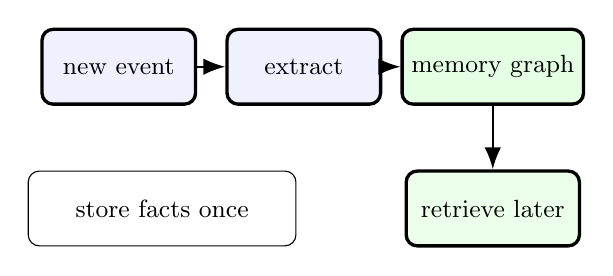
\begin{tikzpicture}[>=Latex, every node/.style={font=\small}]
      \node[stepbox, minimum width=1.95cm] (obs) at (0,1.0) {new event};
      \node[stepbox, minimum width=1.95cm] (ext) at (2.35,1.0) {extract};
      \node[entity2, minimum width=2.2cm] (kg) at (4.75,1.0) {memory graph};
      \node[stepbox2, minimum width=2.2cm] (ret) at (4.75,-0.8) {retrieve later};
      \draw[flowarrow] (obs) -- (ext);
      \draw[flowarrow] (ext) -- (kg);
      \draw[flowarrow] (kg.south) -- (ret.north);
      \node[softbox, minimum width=3.4cm] at (0.55,-0.8) {store facts once};
    \end{tikzpicture}
    \end{center}
  \end{column}
\end{columns}
\plainidea{Graph memory helps an agent stay consistent across many tool calls and long tasks.}
\end{frame}

\begin{frame}{KGs for Explanation}
\keyquestion{Why are graph paths useful when we want the system to explain an answer?}
\begin{center}
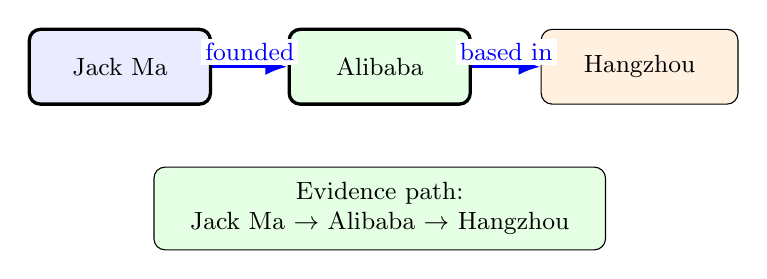
\begin{tikzpicture}[>=Latex, every node/.style={font=\small}]
  \node[entity] (ma) at (0,0) {Jack Ma};
  \node[entity2] (ali) at (3.3,0) {Alibaba};
  \node[note] (hz) at (6.6,0) {Hangzhou};
  \draw[flowarrow, very thick, blue] (ma) -- node[relabel, above]{founded} (ali);
  \draw[flowarrow, very thick, blue] (ali) -- node[relabel, above]{based in} (hz);
  \node[draw, rounded corners, fill=green!10, text width=5.5cm, minimum height=1.05cm, align=center] at (3.3,-1.8) {Evidence path:\\ Jack Ma $\rightarrow$ Alibaba $\rightarrow$ Hangzhou};
\end{tikzpicture}
\end{center}
\plainidea{A graph path is a small, readable explanation. It shows where the answer came from.}
\end{frame}

\begin{frame}{KGs in Multimodal AI}
\keyquestion{How can a graph help when the system uses images and text together?}
\begin{center}
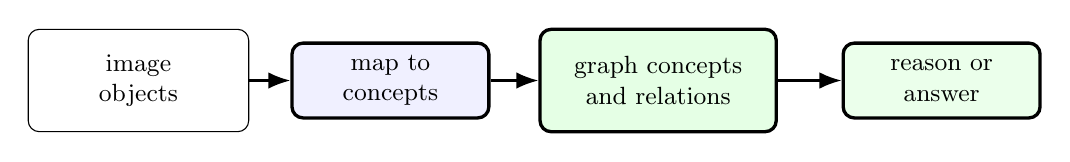
\begin{tikzpicture}[>=Latex, every node/.style={font=\small}]
  \node[softbox, minimum width=2.8cm, minimum height=1.3cm] (img) at (0,0) {image\\ objects};
  \node[stepbox] (map) at (3.2,0) {map to\\ concepts};
  \node[entity2, minimum width=3.0cm, minimum height=1.3cm] (kg) at (6.6,0) {graph concepts\\ and relations};
  \node[stepbox2] (qa) at (10.2,0) {reason or\\ answer};
  \draw[flowarrow] (img) -- (map);
  \draw[flowarrow] (map) -- (kg);
  \draw[flowarrow] (kg) -- (qa);
\end{tikzpicture}
\end{center}
\plainidea{The graph gives the model structured concepts and relations, not just raw pixels or raw words.}
\end{frame}

\begin{frame}{What Is Neuro-Symbolic AI?}
\keyquestion{What do people mean when they say neuro-symbolic AI?}
\begin{columns}[T,onlytextwidth]
  \begin{column}{0.46\textwidth}
    \begin{tcolorbox}[colback=questionbg,colframe=questionframe,boxrule=0.7pt,title=Neural part]
    Good at pattern learning from large data
    \end{tcolorbox}
    \begin{tcolorbox}[colback=plainbg,colframe=plainframe,boxrule=0.7pt,title=Symbolic part]
    Good at explicit structure, rules, and traceable reasoning
    \end{tcolorbox}
  \end{column}
  \begin{column}{0.50\textwidth}
    \begin{center}
    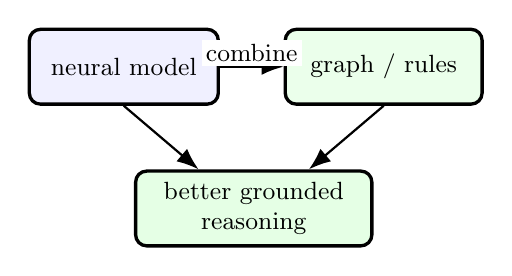
\begin{tikzpicture}[>=Latex, every node/.style={font=\small}]
      \node[stepbox, minimum width=2.4cm] (n) at (0,0.8) {neural model};
      \node[stepbox2, minimum width=2.5cm] (s) at (3.3,0.8) {graph / rules};
      \node[entity2, minimum width=3.0cm] (out) at (1.65,-1.0) {better grounded\\ reasoning};
      \draw[flowarrow] (n) -- node[relabel, above]{combine} (s);
      \draw[flowarrow] (n.south) -- ([xshift=-0.7cm]out.north);
      \draw[flowarrow] (s.south) -- ([xshift=0.7cm]out.north);
    \end{tikzpicture}
    \end{center}
  \end{column}
\end{columns}
\plainidea{Neuro-symbolic AI tries to combine flexible learning with explicit reasoning structure.}
\end{frame}

\begin{frame}{Pattern 1: Neural to Symbolic}
\keyquestion{What happens when a neural model writes facts into a graph?}
\begin{center}
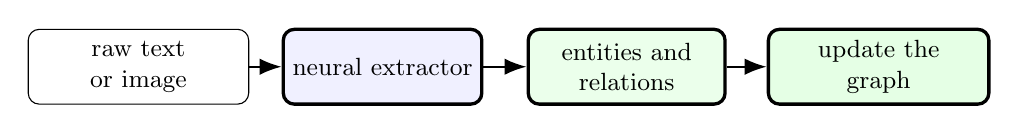
\begin{tikzpicture}[>=Latex, every node/.style={font=\small}]
  \node[softbox, minimum width=2.8cm] (raw) at (0,0) {raw text\\ or image};
  \node[stepbox] (extract) at (3.1,0) {neural extractor};
  \node[stepbox2] (triples) at (6.2,0) {entities and\\ relations};
  \node[entity2, minimum width=2.8cm] (kg) at (9.4,0) {update the\\ graph};
  \draw[flowarrow] (raw) -- (extract);
  \draw[flowarrow] (extract) -- (triples);
  \draw[flowarrow] (triples) -- (kg);
\end{tikzpicture}
\end{center}
\plainidea{Here the neural model reads messy input and turns it into structured graph facts.}
\end{frame}

\begin{frame}{Pattern 2: Symbolic to Neural}
\keyquestion{What happens when a graph gives evidence to a neural model?}
\begin{center}
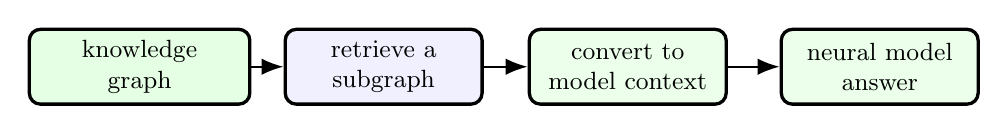
\begin{tikzpicture}[>=Latex, every node/.style={font=\small}]
  \node[entity2, minimum width=2.8cm] (kg) at (0,0) {knowledge\\ graph};
  \node[stepbox] (ret) at (3.1,0) {retrieve a\\ subgraph};
  \node[stepbox2] (ctx) at (6.2,0) {convert to\\ model context};
  \node[stepbox2] (llm) at (9.4,0) {neural model\\ answer};
  \draw[flowarrow] (kg) -- (ret);
  \draw[flowarrow] (ret) -- (ctx);
  \draw[flowarrow] (ctx) -- (llm);
\end{tikzpicture}
\end{center}
\plainidea{Here the graph guides the neural model by supplying explicit facts before the answer is generated.}
\end{frame}

\begin{frame}{Pattern 3: Joint or Constrained}
\keyquestion{Can we make the neural model and the graph influence each other during learning or checking?}
\begin{center}
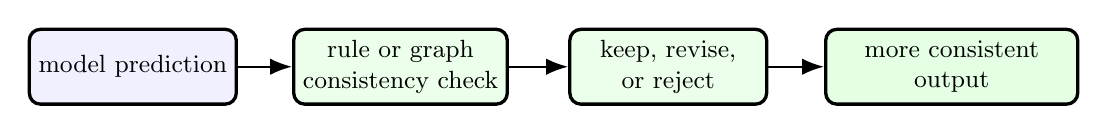
\begin{tikzpicture}[>=Latex, every node/.style={font=\small}]
  \node[stepbox] (pred) at (0,0) {model prediction};
  \node[stepbox2] (check) at (3.4,0) {rule or graph\\ consistency check};
  \node[stepbox2] (repair) at (6.8,0) {keep, revise,\\ or reject};
  \node[entity2, minimum width=3.2cm] (out) at (10.4,0) {more consistent\\ output};
  \draw[flowarrow] (pred) -- (check);
  \draw[flowarrow] (check) -- (repair);
  \draw[flowarrow] (repair) -- (out);
\end{tikzpicture}
\end{center}
\plainidea{This pattern uses graph rules or constraints to catch weak outputs and improve consistency.}
\end{frame}

\begin{frame}{What Do Recent Reviews Report?}
\keyquestion{When people review many neuro-symbolic papers together, what trends do they keep finding?}
\begin{columns}[T,onlytextwidth]
  \begin{column}{0.48\textwidth}
    \begin{tcolorbox}[colback=green!6,colframe=green!50!black,boxrule=0.7pt,title=Often reported benefits]
    \begin{itemize}
      \item better explainability
      \item better multi-hop reasoning
      \item stronger grounding
    \end{itemize}
    \end{tcolorbox}
  \end{column}
  \begin{column}{0.48\textwidth}
    \begin{tcolorbox}[colback=orange!10,colframe=orange!70!black,boxrule=0.7pt,title=Often reported problems]
    \begin{itemize}
      \item incomplete or noisy graphs
      \item expensive maintenance
      \item evaluation still inconsistent
    \end{itemize}
    \end{tcolorbox}
  \end{column}
\end{columns}
\plainidea{The idea is promising, but the graph still has to be clean, maintained, and evaluated well.}
\end{frame}

\begin{frame}{A Simple Practical Pipeline}
\keyquestion{If we want to deploy a graph-backed AI system, what is a simple end-to-end workflow?}
\begin{center}
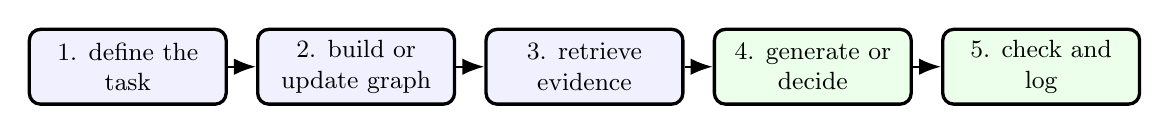
\begin{tikzpicture}[>=Latex, every node/.style={font=\small}]
  \node[stepbox] (goal) at (0,0) {1. define the\\ task};
  \node[stepbox] (build) at (2.9,0) {2. build or\\ update graph};
  \node[stepbox] (ret) at (5.8,0) {3. retrieve\\ evidence};
  \node[stepbox2] (gen) at (8.7,0) {4. generate or\\ decide};
  \node[stepbox2] (check) at (11.6,0) {5. check and\\ log};
  \draw[flowarrow] (goal) -- (build);
  \draw[flowarrow] (build) -- (ret);
  \draw[flowarrow] (ret) -- (gen);
  \draw[flowarrow] (gen) -- (check);
\end{tikzpicture}
\end{center}
\plainidea{The graph is one stage in a full pipeline, not a magic box by itself.}
\end{frame}

\begin{frame}{Operational Challenges}
\keyquestion{What usually makes a graph-backed AI system difficult to run in practice?}
\small
\begin{columns}[T,onlytextwidth]
  \begin{column}{0.48\textwidth}
    \begin{tcolorbox}[colback=red!6,colframe=red!60!black,boxrule=0.7pt,title=Data problems]
    entity-linking errors, stale facts, missing source
    \end{tcolorbox}
    \begin{tcolorbox}[colback=orange!10,colframe=orange!70!black,boxrule=0.7pt,title=System problems]
    retrieval latency, higher cost, harder monitoring
    \end{tcolorbox}
  \end{column}
  \begin{column}{0.48\textwidth}
    \begin{tcolorbox}[colback=blue!6,colframe=blue!60!black,boxrule=0.7pt,title=Policy problems]
    access control, privacy, bias, auditing
    \end{tcolorbox}
    \begin{tcolorbox}[colback=green!6,colframe=green!50!black,boxrule=0.7pt,title=Teaching message]
    strong reasoning still needs careful engineering
    \end{tcolorbox}
  \end{column}
\end{columns}
\vspace{-0.3em}
\plainidea{Many failures come from bad data, weak controls, or slow retrieval design, not only from the model.}
\end{frame}

\setslideref{References listed at end}
\begin{frame}{What Is MCP and Why Does It Matter?}
\keyquestion{What is MCP, and why do modern agent systems need it?}
\begin{tcolorbox}[colback=questionbg,colframe=questionframe,boxrule=0.7pt,title=Definition]
MCP stands for \textbf{Model Context Protocol}. It is a standard way for an AI application to connect to external tools, data, and prompts.
\end{tcolorbox}
\vspace{0.2em}
\begin{center}
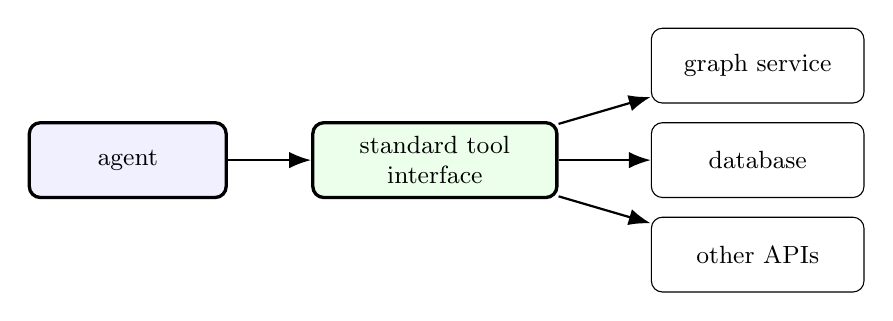
\begin{tikzpicture}[>=Latex, every node/.style={font=\small}]
  \node[stepbox] (agent) at (0,0) {agent};
  \node[stepbox2, minimum width=3.1cm] (mcp) at (3.9,0) {standard tool\\ interface};
  \node[softbox] (kg) at (8.0,1.2) {graph service};
  \node[softbox] (db) at (8.0,0) {database};
  \node[softbox] (api) at (8.0,-1.2) {other APIs};
  \draw[flowarrow] (agent) -- (mcp);
  \draw[flowarrow] (mcp) -- (kg);
  \draw[flowarrow] (mcp) -- (db);
  \draw[flowarrow] (mcp) -- (api);
\end{tikzpicture}
\end{center}
\plainidea{A standard tool interface makes agent systems easier to connect, swap, and govern.}
\end{frame}

\setslideref{References listed at end}
\begin{frame}{MCP Core Roles}
\keyquestion{What are the main parts in a simple MCP-style setup?}
\begin{center}
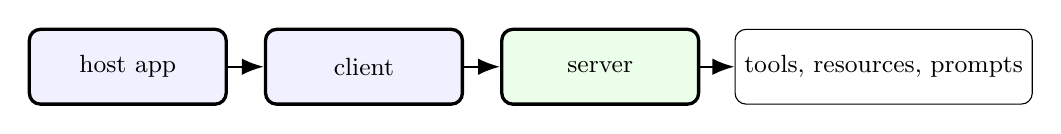
\begin{tikzpicture}[>=Latex, every node/.style={font=\small}]
  \node[stepbox] (host) at (0,0) {host app};
  \node[stepbox] (client) at (3.0,0) {client};
  \node[stepbox2] (server) at (6.0,0) {server};
  \node[softbox, minimum width=3.0cm] (tools) at (9.6,0) {tools, resources, prompts};
  \draw[flowarrow] (host) -- (client);
  \draw[flowarrow] (client) -- (server);
  \draw[flowarrow] (server) -- (tools);
\end{tikzpicture}
\end{center}
\plainidea{The host runs the assistant, the client connects, and the server exposes usable capabilities.}
\end{frame}

\setslideref{References listed at end}
\begin{frame}{MCP Request Flow}
\keyquestion{What happens from a user question to a final grounded answer?}
\begin{center}
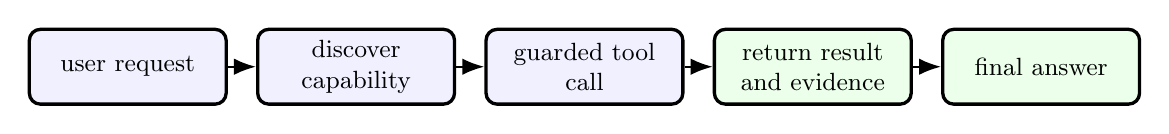
\begin{tikzpicture}[>=Latex, every node/.style={font=\small}]
  \node[stepbox] (q) at (0,0) {user request};
  \node[stepbox] (discover) at (2.9,0) {discover\\ capability};
  \node[stepbox] (call) at (5.8,0) {guarded tool\\ call};
  \node[stepbox2] (res) at (8.7,0) {return result\\ and evidence};
  \node[stepbox2] (ans) at (11.6,0) {final answer};
  \draw[flowarrow] (q) -- (discover);
  \draw[flowarrow] (discover) -- (call);
  \draw[flowarrow] (call) -- (res);
  \draw[flowarrow] (res) -- (ans);
\end{tikzpicture}
\end{center}
\plainidea{The useful idea is simple: discover the right tool, call it safely, then answer with returned evidence.}
\end{frame}

\setslideref{References listed at end}
\begin{frame}{MCP Security and Governance}
\keyquestion{What controls do we need before an agent is allowed to use real tools?}
\begin{columns}[T,onlytextwidth]
  \begin{column}{0.48\textwidth}
    \begin{tcolorbox}[colback=questionbg,colframe=questionframe,boxrule=0.7pt,title=Before the call]
    allowlists, role checks, input checks
    \end{tcolorbox}
    \begin{tcolorbox}[colback=plainbg,colframe=plainframe,boxrule=0.7pt,title=During the call]
    secrets protection, bounded scope, timeouts
    \end{tcolorbox}
  \end{column}
  \begin{column}{0.48\textwidth}
    \begin{tcolorbox}[colback=notationbg,colframe=notationframe,boxrule=0.7pt,title=After the call]
    logs, audit trails, policy review
    \end{tcolorbox}
  \end{column}
\end{columns}
\plainidea{Good tool use is not just about capability. It is also about permission, safety, and traceability.}
\end{frame}

\setslideref{References listed at end}
\begin{frame}{Why Multi-Agent Systems?}
\keyquestion{Why use more than one agent instead of one very large prompt?}
\begin{center}
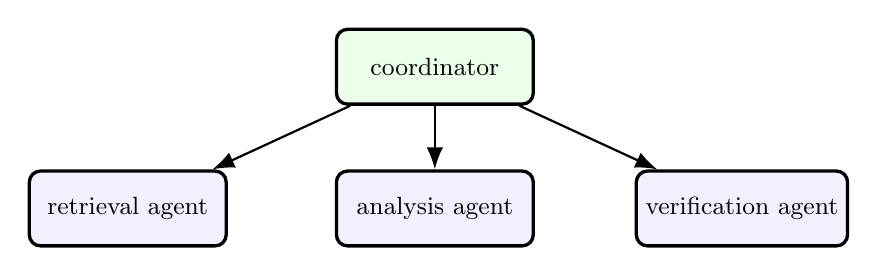
\begin{tikzpicture}[>=Latex, every node/.style={font=\small}]
  \node[stepbox2] (sup) at (4.7,1.8) {coordinator};
  \node[stepbox] (r) at (0.8,0) {retrieval agent};
  \node[stepbox] (a) at (4.7,0) {analysis agent};
  \node[stepbox] (v) at (8.6,0) {verification agent};
  \draw[flowarrow] (sup) -- (r);
  \draw[flowarrow] (sup) -- (a);
  \draw[flowarrow] (sup) -- (v);
\end{tikzpicture}
\end{center}
\plainidea{Multiple agents can split work, specialise roles, and check each other.}
\end{frame}

\setslideref{References listed at end}
\begin{frame}{Pattern: Supervisor and Workers}
\keyquestion{What is the simplest multi-agent pattern to understand first?}
\begin{center}
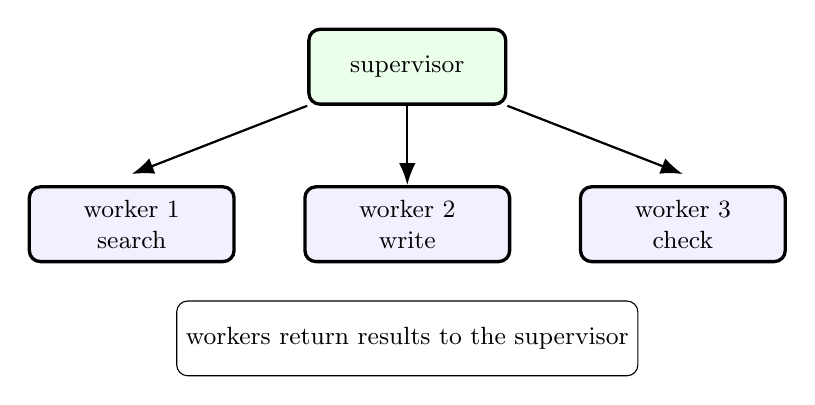
\begin{tikzpicture}[>=Latex, every node/.style={font=\small}]
  \node[stepbox2] (sup) at (4.6,2.0) {supervisor};
  \node[stepbox, minimum width=2.6cm] (w1) at (1.1,0) {worker 1\\ search};
  \node[stepbox, minimum width=2.6cm] (w2) at (4.6,0) {worker 2\\ write};
  \node[stepbox, minimum width=2.6cm] (w3) at (8.1,0) {worker 3\\ check};
  \draw[flowarrow] (sup.south west) -- ([yshift=4pt]w1.north);
  \draw[flowarrow] (sup.south) -- (w2.north);
  \draw[flowarrow] (sup.south east) -- ([yshift=4pt]w3.north);
  \node[softbox, minimum width=4.1cm] at (4.6,-1.45) {workers return results to the supervisor};
    \end{tikzpicture}
\end{center}
\plainidea{The supervisor assigns work, workers do one focused job, and the supervisor combines the results.}
\end{frame}

\setslideref{References listed at end}
\begin{frame}{Pattern: Planner, Executor, Critic}
\keyquestion{How can we separate planning, doing, and checking?}
\begin{center}
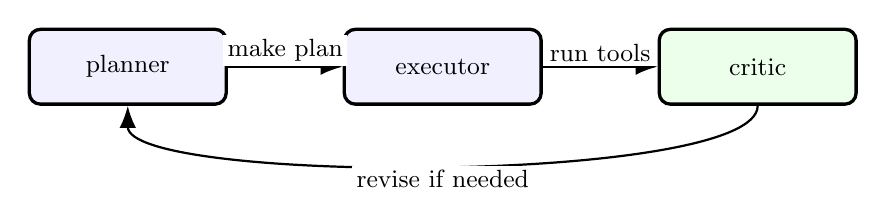
\begin{tikzpicture}[>=Latex, every node/.style={font=\small}]
  \node[stepbox] (plan) at (0,0) {planner};
  \node[stepbox] (exec) at (4.0,0) {executor};
  \node[stepbox2] (crit) at (8.0,0) {critic};
  \draw[flowarrow] (plan) -- node[relabel, above]{make plan} (exec);
  \draw[flowarrow] (exec) -- node[relabel, above]{run tools} (crit);
  \draw[flowarrow] (crit.south) .. controls +(down:1.0cm) and +(down:1.0cm) .. node[relabel, below]{revise if needed} (plan.south);
\end{tikzpicture}
\end{center}
\plainidea{This pattern is useful when we want the system to plan first and then check its own work.}
\end{frame}

\setslideref{References listed at end}
\begin{frame}{What Is Agent-to-Agent (A2A)?}
\keyquestion{What changes when one agent talks directly to another independent agent?}
\begin{columns}[T,onlytextwidth]
  \begin{column}{0.44\textwidth}
    \begin{tcolorbox}[colback=questionbg,colframe=questionframe,boxrule=0.7pt,title=Simple idea]
    One agent asks another agent for help on a task it cannot or should not do alone.
    \end{tcolorbox}
  \end{column}
  \begin{column}{0.52\textwidth}
    \begin{center}
    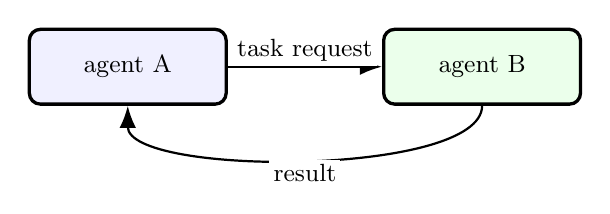
\begin{tikzpicture}[>=Latex, every node/.style={font=\small}]
      \node[stepbox] (a1) at (0,0) {agent A};
      \node[stepbox2] (a2) at (4.5,0) {agent B};
      \draw[flowarrow] (a1) -- node[relabel, above]{task request} (a2);
      \draw[flowarrow] (a2.south) .. controls +(down:0.9cm) and +(down:0.9cm) .. node[relabel, below]{result} (a1.south);
    \end{tikzpicture}
    \end{center}
  \end{column}
\end{columns}
\plainidea{A2A is about coordination across agents, not just tool use inside one agent.}
\end{frame}

\setslideref{References listed at end}
\begin{frame}{A2A Handoff Sequence}
\keyquestion{What are the basic steps in a safe agent-to-agent handoff?}
\begin{center}
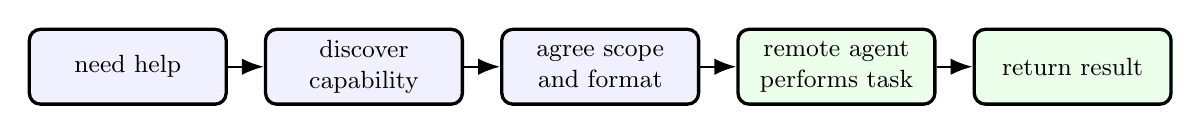
\begin{tikzpicture}[>=Latex, every node/.style={font=\small}]
  \node[stepbox] (need) at (0,0) {need help};
  \node[stepbox] (discover) at (3.0,0) {discover\\ capability};
  \node[stepbox] (agree) at (6.0,0) {agree scope\\ and format};
  \node[stepbox2] (run) at (9.0,0) {remote agent\\ performs task};
  \node[stepbox2] (return) at (12.0,0) {return result};
  \draw[flowarrow] (need) -- (discover);
  \draw[flowarrow] (discover) -- (agree);
  \draw[flowarrow] (agree) -- (run);
  \draw[flowarrow] (run) -- (return);
\end{tikzpicture}
\end{center}
\plainidea{A good handoff makes the scope clear before work starts, so the result is easier to trust and reuse.}
\end{frame}

\setslideref{References listed at end}
\begin{frame}{Tool-Choice Reasoning}
\keyquestion{How does a modern assistant decide what to do next?}
\begin{center}
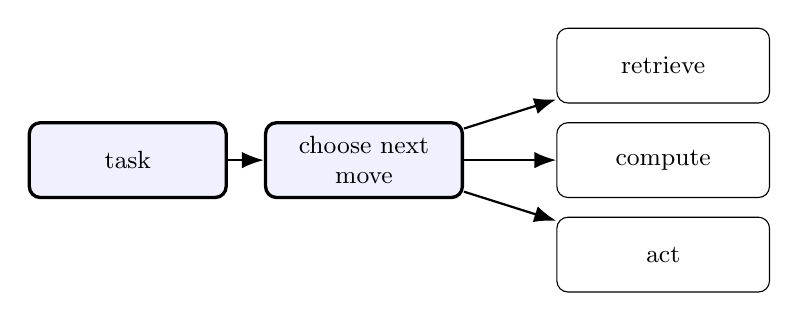
\begin{tikzpicture}[>=Latex, every node/.style={font=\small}]
  \node[stepbox] (q) at (0,0) {task};
  \node[stepbox] (think) at (3.0,0) {choose next\\ move};
  \node[softbox] (r1) at (6.8,1.2) {retrieve};
  \node[softbox] (r2) at (6.8,0) {compute};
  \node[softbox] (r3) at (6.8,-1.2) {act};
  \draw[flowarrow] (q) -- (think);
  \draw[flowarrow] (think) -- (r1);
  \draw[flowarrow] (think) -- (r2);
  \draw[flowarrow] (think) -- (r3);
\end{tikzpicture}
\end{center}
\plainidea{A strong assistant does not call tools randomly. It chooses whether to retrieve, compute, or act.}
\end{frame}

\setslideref{References listed at end}
\begin{frame}{Coding-Agent Style Runtime Preview}
\keyquestion{What simple runtime pattern will we study in more detail tomorrow?}
\begin{center}
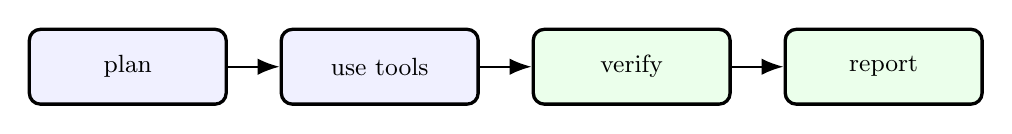
\begin{tikzpicture}[>=Latex, every node/.style={font=\small}]
  \node[stepbox] (plan) at (0,0) {plan};
  \node[stepbox] (tool) at (3.2,0) {use tools};
  \node[stepbox2] (check) at (6.4,0) {verify};
  \node[stepbox2] (report) at (9.6,0) {report};
  \draw[flowarrow] (plan) -- (tool);
  \draw[flowarrow] (tool) -- (check);
  \draw[flowarrow] (check) -- (report);
\end{tikzpicture}
\end{center}
\plainidea{Tomorrow we will look closely at coding agents, but the basic runtime idea is already here: plan, use tools, verify, report.}
\end{frame}

\begin{frame}{Domain Snapshot: Internal Knowledge Copilot}
\keyquestion{What could a graph-backed enterprise assistant look like in practice?}
\begin{center}
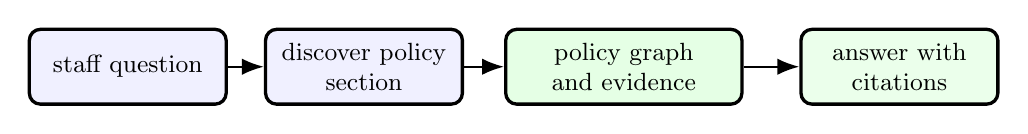
\begin{tikzpicture}[>=Latex, every node/.style={font=\small}]
  \node[stepbox] (q) at (0,0) {staff question};
  \node[stepbox] (disc) at (3.0,0) {discover policy\\ section};
  \node[entity2, minimum width=3.0cm] (kg) at (6.3,0) {policy graph\\ and evidence};
  \node[stepbox2] (ans) at (9.8,0) {answer with\\ citations};
  \draw[flowarrow] (q) -- (disc);
  \draw[flowarrow] (disc) -- (kg);
  \draw[flowarrow] (kg) -- (ans);
\end{tikzpicture}
\end{center}
\begin{itemize}
  \item retrieve only relevant policy evidence
  \item keep access control and redaction rules
  \item return citations with the answer
\end{itemize}
\plainidea{The graph helps the assistant answer with evidence and policy structure, not just fluent text.}
\end{frame}

\begin{frame}{Transition to Day 5}
\keyquestion{What comes after standards, coordination, and graph-backed agent design?}
\begin{itemize}
  \item Today focused on architecture patterns for modern AI systems.
  \item Tomorrow focuses on coding agents in more detail.
  \item We will look more closely at trust, tool use, verification, and safe execution.
\end{itemize}
\plainidea{Day 4 showed the system-level picture. Day 5 goes deeper into one important case: coding agents.}
\end{frame}

\setslideref{End-of-lecture recap}
\begin{frame}{Scope Boundary for This Block}
\keyquestion{What are we deliberately not doing in Block 3?}
\begin{itemize}
  \item We focus on how graphs improve AI behaviour.
  \item We do not go deep into query-language syntax such as SPARQL or Cypher.
  \item In this module, query syntax is less important than reasoning flow, grounding, and system design.
\end{itemize}
\plainidea{For this module, think first about the reasoning system. Treat low-level query syntax as an implementation detail.}
\end{frame}

\setslideref{End-of-lecture recap}
\begin{frame}{Key Takeaways}
\begin{itemize}
  \item Knowledge graphs improve retrieval, memory, reasoning, and explanation.
  \item Neuro-symbolic systems mix flexible learning with explicit structure.
  \item MCP, multi-agent patterns, and A2A help organise modern tool-using systems.
  \item Strong reasoning systems still need evidence, guardrails, and good engineering practice.
\end{itemize}
\plainidea{The big theme is grounding: modern AI becomes more useful when its actions and answers stay connected to explicit evidence and clear system structure.}
\end{frame}

\setslideref{Exercise prompt for class discussion}
\begin{frame}{In-Class Exercises}
\exercisebreakcontent{Use the exercise time to decide where graph structure adds the most value inside a modern AI pipeline.}
\end{frame}

\setslideref{Practice exercises listed on this slide}
\begin{frame}{Further Study}
\begin{itemize}
  \item Read Poole Chapters 16 and 17, and revisit AIMA Chapter 10.
  \item Practice: Poole Ch.16, Exercises 16.3, 16.4, and 16.5.
  \item Practice: Poole Ch.17, Exercises 17.4, 17.5, and 17.8.
  \item AIMA knowledge-representation exercise page: 7, 8, 26, and 28.
  \item Focus on graph-backed retrieval, structured evidence, and how explicit relations change the reasoning flow.
\end{itemize}
\end{frame}

\setslideref{Full references listed on this slide}
\begin{frame}[allowframebreaks]{Full References for This Lecture}
\footnotesize
\begin{thebibliography}{9}
\bibitem{aima10}
Russell, S. and Norvig, P. (2021).
\newblock \textit{Artificial Intelligence: A Modern Approach} (4th ed.).
\newblock Pearson. Chapter 10, pp.~314--343.

\bibitem{poole16_17}
Poole, D. L. and Mackworth, A. K. (2023).
\newblock \textit{Artificial Intelligence: Foundations of Computational Agents} (3rd ed.).
\newblock Cambridge University Press. Chapters 16--17, pp.~701--766.

\bibitem{delong2024}
DeLong, L. N., Mir, R. F. and Fleuriot, J. D. (2024).
\newblock Neurosymbolic AI for reasoning over knowledge graphs: A survey.
\newblock \textit{IEEE Transactions on Neural Networks and Learning Systems}.
\newblock DOI: \url{https://doi.org/10.1109/TNNLS.2024.3420218}

\bibitem{colelough2025}
Colelough, E. and Regli, W. C. (2025).
\newblock Neuro-Symbolic AI in 2024: A systematic review.
\newblock \textit{arXiv preprint} arXiv:2501.05435.
\newblock DOI: \url{https://doi.org/10.48550/arXiv.2501.05435}

\bibitem{nawaz2025}
Nawaz, W., Shah, M. A., Kim, Y. G. and Kim, M. (2025).
\newblock A review of neuro-symbolic AI integrating reasoning and learning for advanced cognitive systems.
\newblock \textit{Intelligent Systems with Applications}, 29, 200541.
\newblock DOI: \url{https://doi.org/10.1016/j.iswa.2025.200541}

\bibitem{hakim2026}
Hakim, M. A., Nawaz, W., Ahmed, K. T. and Shah, M. A. (2026).
\newblock Neuro-Symbolic Agentic AI: Architectures, integration patterns, applications, and open challenges.
\newblock \textit{Computer Science Review}, 60, 100902.
\newblock DOI: \url{https://doi.org/10.1016/j.cosrev.2026.100902}

\bibitem{mcp}
Anthropic.
\newblock Model Context Protocol specification.
\newblock \url{https://modelcontextprotocol.io/specification/}

\bibitem{a2a}
Google.
\newblock Agent-to-Agent (A2A) protocol documentation.
\newblock \url{https://a2a-protocol.org/dev/}

\bibitem{openaiagentssdk}
OpenAI.
\newblock OpenAI Agents Python documentation.
\newblock \url{https://openai.github.io/openai-agents-python/}

\bibitem{codexplatform}
OpenAI.
\newblock Codex product page.
\newblock \url{https://openai.com/codex/}

\bibitem{openclaw}
OpenClaw.
\newblock OpenClaw documentation.
\newblock \url{https://getopenclaw.ai/docs}
\end{thebibliography}
\end{frame}

\end{document}
